\documentclass[pageno]{jpaper}

% Change to current semester and year, e.g.:
% \newcommand{\IWreport}{Spring 2020}
\newcommand{\IWreport}{Spring 2021}
\newcommand{\quotes}[1]{``#1''}


\widowpenalty=9999

\usepackage[normalem]{ulem}
\usepackage{pgf-pie}
\usepackage{enumitem}
\usepackage{caption}
\usepackage[newfloat]{minted}
\usepackage{keystroke}
\captionsetup[listing]{position=top}

\begin{document}

\title{Teaching Graph Traversal Visually}

\author{William Svoboda\\Adviser: David Walker}

\date{}
\maketitle

\thispagestyle{empty}
\doublespacing
\begin{abstract}
Visual learning presents an opportunity to more effectively teach computer science fundamentals. However, existing solutions are unable to both facilitate user interaction and focus on implementation. This paper describes an assignment and programming framework for teaching graph traversal algorithms. Visualization tools are contextualized as a way to improve the learning experience, and an evaluation of the project with real students is discussed.
\end{abstract}

\section{Introduction}

Before the theory and practice of computing can be understood, it follows that they must first be taught. Computer science is now an unshakeable part of modern society, and its applications shape our lives in fundamental ways. Beyond the complexity of these applications, however, is the difficulty of understanding computer science itself. As our world moves ever closer to a digital future, it is critical that people are given a solid foundation in computing. Computer science, however, is an ocean that is as wide as it is deep. Different areas of computer science may benefit from different ways of teaching.

My project falls within one of these niches. Graph theory is a core focus area of computer science, and it has proven to be a valuable way of understanding real-world problems. Graphs, for example, can be contextualized to represent networks, relationships, navigation, and more. While many parts of computer science might benefit from visualization, the nature of graph theory makes it an ideal candidate for visual teaching. Visualization is not a substitute for formal theory, but it does enable faster communication and understanding.

The goal of my independent work project was to teach graph traversal algorithms in a visual way. In this paper, I describe an interactive assignment using the Python programming language that accomplishes this goal.

\section{Problem Background}

A graph describes a set of \emph{nodes} and the relationships between them~\cite{graph}. As stated in the introduction, graph theory is widely applicable to real-world problems. A connection between any pair of nodes, also called an \emph{edge}, might be contextualized to represent a path, a transaction, or any number of other relationships. Edges can be classified as either directed or undirected. While an undirected edge implies that the relationship between two nodes is reciprocal, a directed edge occurs when the relationship is one-way~\cite{graph}. Graphs in turn might be weighted (when each edge is assigned a numeric value) or directed (when each edge has a direction)~\cite{graph}. While graph theory is much broader than this limited description, for the purpose of this project I focused on graphs that were both unweighted and undirected.

Because my independent work concerned itself specifically with the \emph{traversal} of graphs, it was necessary to choose relevant algorithms which could be taught to students. Two of the most well-known algorithms, depth-first search and breadth-first search, presented excellent candidates for an assignment given their simplicity and popularity.

Depth-first search has been formally investigated since at least the 19th century~\cite{dfs}, but the underlying strategy is perhaps even older.\footnote{In the Greek myth of Theseus and the Minotaur, the hero Theseus is given a ball of string by his lover Ariadne in order to navigate the Minotaur's Labyrinth. After reaching a dead end, Theseus could use the string to retrace his steps and find a new path to search.} The algorithm starts at a root node before exploring as far as possible down a given branch. If the end of a branch is reached, the algorithm backtracks and checks the next possible branch~\cite{dfs}. In this way, depth-first search can be used to find all nodes connected to a given vertex.

In comparison, breadth-first search takes the opposite approach. The algorithm explores each neighbor of the current node before moving down the next branch~\cite{bfs}. While breadth-first search was initially developed in 1945 by the German scientist Konrad Zuse, a similar strategy was used by Edward Moore in 1959 to find the shortest path through a maze~\cite{bfs}.\footnote{Interestingly, it is not possible to use unmodified depth-first search to find the shortest path between two nodes~\cite{suboptimal}. While a depth-first approach can be used to find \emph{a path}, this is not guaranteed to be the shortest possible one in the graph.}

Depending on the properties of a particular graph, it is possible to use more sophisticated strategies. However, I focused on creating an assignment suitable for a wide range of experience levels. As a result, only depth-first search and breadth-first search were selected for the final specification.

\section{Related Work}

Visual learning has long been explored by computer scientists. One popular solution, Scratch~\cite{scratch}, was created in 2003 by MIT. Scratch is a visual programming language, where logic is represented with blocks that can be arranged to create different applications. Scratch has found great success as a teaching tool for new programmers of all ages, and it continues to have a large and active community worldwide. 

Visualizing algorithms specifically, including those for graph traversal, is also an area of active development. Two websites, VisuAlgo~\cite{visualgo} and David Galles's \emph{Data Structure Visualizations}~\cite{usf}, both provide a way to view algorithms online. Users can trace through the operation of a given algorithm, setting the visualization speed and other options such as input size.

These examples, however, do not provide a definitive solution. To be more specific, there is room for a teaching framework that is both interactive and applicable to modern toolsets. While Scratch effectively teaches basic programming logic, its features do not compare to languages like Java, Python, and C that might be used in more advanced settings. VisuAlgo and Galles's offerings are well-suited to pure explanation, but they do not focus on the actual implementation of each algorithm. My project aims to fill both of these gaps.

\section{Approach}

Creating an interactive programming assignment requires two distinct—but interconnected—areas of work. The first is the actual implementation of the project. This required not only implementing the visualization of each algorithm, but also facilitating student interaction such that the algorithms could be taught programmatically. To accomplish these tasks, I intended to find a programming language that was both powerful and accessible to new programmers. This would reduce the difficulty of interfacing between project-written and student-written code, alongside reducing the overall complexity of the codebase.

The second is the contextualization of the project as an assignment. This entailed adapting the project implementation to a formal assignment specification. A student taking the assignment would need to be walked through each of the two selected traversal algorithms (depth-first search and breadth-first search) in a structured way. Moreover, there would need to be an assessment of the student to determine their mastery of the material.

These two areas of work logically follow each other. In order to develop the assignment specifications, it was necessary to first ensure the key implementation details were in place. With visualization at the core of the project, students would be better equipped to understand, analyze, and ultimately write their own implementation of each algorithm.

\section{Implementation}

\subsection{Tool Selection}

Because my project focused on both visualization and user interaction, the choice of development environment was critical. Game engines are a natural fit, because they provide a framework that is well-suited to handling both graphics and user input. After some consideration of other software, namely the Unity game engine, I selected Pygame~\cite{pygame} as the tool of choice.

This decision went hand-in-hand with the choice of programming language. Pygame is a set of Python modules that wrap around the SDL graphics library~\cite{pygame}. Python, in comparison to languages like C, offers a high-level syntax that makes it easy to write powerful, concise code. Python is also one of the most popular programming languages today. This meant that students could apply their learning to future work where Python would likely appear again. By using Python and Pygame together, it was possible to use the same programming language throughout the project. Any code written by students would be directly compatible with the visualization software. Finally, and perhaps most importantly, both Python and Pygame are multi-platform. This meant that students would be able complete the assignment no matter what operating system they used, and very little platform-specific instructions needed to be written.

The final application and assignment are bundled together as a single Git repository and hosted on GitHub. Git is a proven and widely-adopted solution for version control, and GitHub makes it possible to host and access Git repositories online. Using both of these tools together makes it easy to access all necessary files. Students would be able to make their own copy of the repository, by either forking it or using GitHub's \emph{template repository} feature. During the assignment, students would be able to work on their own computers by using Git to clone the repository locally. This process also had the added benefit of streamlining how students would submit their work. In particular, submission could be handled by simply pushing all changes to the remote repository on GitHub.

The actual assignment specification was written in Markdown, a lightweight text-markup language. Markdown is flexible enough to capture elements like images, block quotations, and code snippets. While Markdown is intended to be processed or converted to another format like HTML, the language's readability and portability make it perfect for authoring rich text~\cite{markdown}. GitHub natively supports rendering Markdown, allowing students to view the final document online as part of the assignment repository. 

To offer an alternative way to access this specification, a website was created to host the same content as the Markdown document on GitHub. The website takes advantage of \emph{GitHub Pages}, a service offered by GitHub for hosting static websites. By default, GitHub Pages will use a repository's \texttt{README.md} as the index page of the site. Because the assignment specification was written in this file, a webpage with the same contents could be generated automatically using any of the built-in themes.

\subsection{ Algorithm Visualization}

The visualization of each graph traversal algorithm is critical to the final product, with all other work depending on its functionality. The visualizer software is written as a single Python script, \texttt{visualizer.py}, and is the main application a student interacts with during the assignment. The visualizer is responsible for three primary tasks:

\begin{enumerate}[label=\textbf{\arabic*.},leftmargin=3cm,font=\textnormal]
\item \emph{Loading Pygame and initializing each Pygame module}
\item \emph{Reading user arguments from the terminal}
\item \emph{Running the main game loop and managing the overall game state}
\end{enumerate}

The visualizer uses the same graph each time the program is run by the student. This graph is presented visually as a regular grid that is 20 cells long and 20 cells wide. The hope was that a grid would make the distances between nodes more apparent, alongside better contextualizing an algorithm like breadth-first search and its use in pathfinding. The graph is represented internally as a two-dimensional array of nodes, which in turn use a \texttt{Node} class contained in \texttt{visualizer.py}. Listing~\ref{lst:node} gives an overview of the \texttt{Node} class and its functions.

\begin{listing}[hbt]
\centering
\begin{minipage}{0.8\textwidth}%
\linespread{1.0}
\caption{Overview of the \texttt{Node} class}
\begin{minted}[linenos,frame=lines,escapeinside=||]{python}
# A single vertex in the graph
class Node:
	# All possible node types
	class NodeType(Enum):
		UNBLOCKED = auto()
		BLOCKED = auto()
		START = auto()
		GOAL = auto()
	# Create a new node
	def __init__(self, x, y) -> None:
		# Position on screen
		self.x = x
		self.y = y
		# Neighboring vertices
		self.neighbors = []
		# Type of node
		self.type = self.NodeType.UNBLOCKED
	# Draw the node on the screen
	def draw(self, screen):
	|\ldots|
	# Connect the node to each of its neighbors
	def addNeighbors(self, graph):
	|\ldots|
\end{minted}
\label{lst:node}
\end{minipage}
\end{listing}

Each individual \texttt{Node} contains a state that represents its specific type. Nodes in the graph can be either \texttt{BLOCKED} or \texttt{UNBLOCKED}, signifying whether or not a given \texttt{Node} can be accessed during traversal. Depending on user input, a given \texttt{Node} might change from one type to another. Two additional types, \texttt{START} and \texttt{GOAL}, are used to declare a unique start and end point in the graph. These types are declared within the \texttt{NodeType} class, which is internal to \texttt{Node} and which uses enumeration to efficiently store each possible state.

The \texttt{Node} class also contains two helper functions which are used throughout the visualizer. The first function, \texttt{draw()}, takes a Pygame \texttt{Surface} as input and updates it. The \texttt{draw()} function is used to essentially draw a given node to the game window using its position and the appropriate color for its \texttt{NodeType}. Listing~\ref{lst:draw} illustrates the logic used for drawing a particular node.

\begin{listing}[hbt]
\centering
\begin{minipage}{0.8\textwidth}%
\linespread{1.0}
\caption{The \texttt{draw()} function}
\begin{minted}[linenos,frame=lines,escapeinside=||]{python}
# Draw the node on the screen
def draw(self, screen):
	color = None
	if self.type == self.NodeType.UNBLOCKED:
		color = WHITE
	elif self.type == self.NodeType.BLOCKED:
		color = BLACK
	elif self.type == self.NodeType.START:
		color = RED
	elif self.type == self.NodeType.GOAL:
		color = BLUE
	pygame.draw.rect(screen, color, 
		(self.x * w + BORDER, 
		self.y * h + BORDER, 
		w - BORDER, 
		h - BORDER))
	pygame.display.update()
\end{minted}
\label{lst:draw}
\end{minipage}
\end{listing}

While Pygame does allow an optional \texttt{width} parameter to be passed when drawing rectangles, I found this to be unsuitable for drawing the grid. The edge lines produced using this method are free to expand beyond the actual borders of the rectangle, resulting in overlap and graphical inconsistencies between grid cells. As a quick solution, a global \texttt{BORDER} variable was declared at the top of \texttt{visualizer.py}. The larger the value of \texttt{BORDER}, the smaller the size of each node on the screen. In this way the color of the background can be used as a visual separator, given that it is set to a unique color.

Because nodes in the grid can have up to four neighbors (one in each of the cardinal directions), each \texttt{Node} also maintains a list of neighboring nodes. The second helper function, \texttt{addNeighbors()}, is called at the start of the visualization. Using the size of the grid as a guide, it checks for adjacent unblocked nodes and adds them to the list of neighbors.

\subsection{User Interaction}

When using the visualization software, a student's entry point is through the terminal. The \texttt{argparse} module was chosen to read command line arguments, because it handles invalid input from the user and is part of Python's standard library. Students are given the option of running the visualizer with a particular algorithm (either depth-first search or breadth-first search). Additionally, the behavior of the visualizer can be changed when running each algorithm. Students can choose to either demonstrate a particular algorithm or test their own implementation against the reference solution stored in \texttt{visualizer.py}. The demonstration is different for each algorithm. When running depth-first-search, the visualizer finds all reachable nodes from the root. When running breadth-first search, the visualizer instead finds the shortest path to the goal node and then draws it on screen. Figure~\ref{fig:argparse} illustrates basic interaction with the visualizer using the terminal.

\begin{figure}[H]
\centering
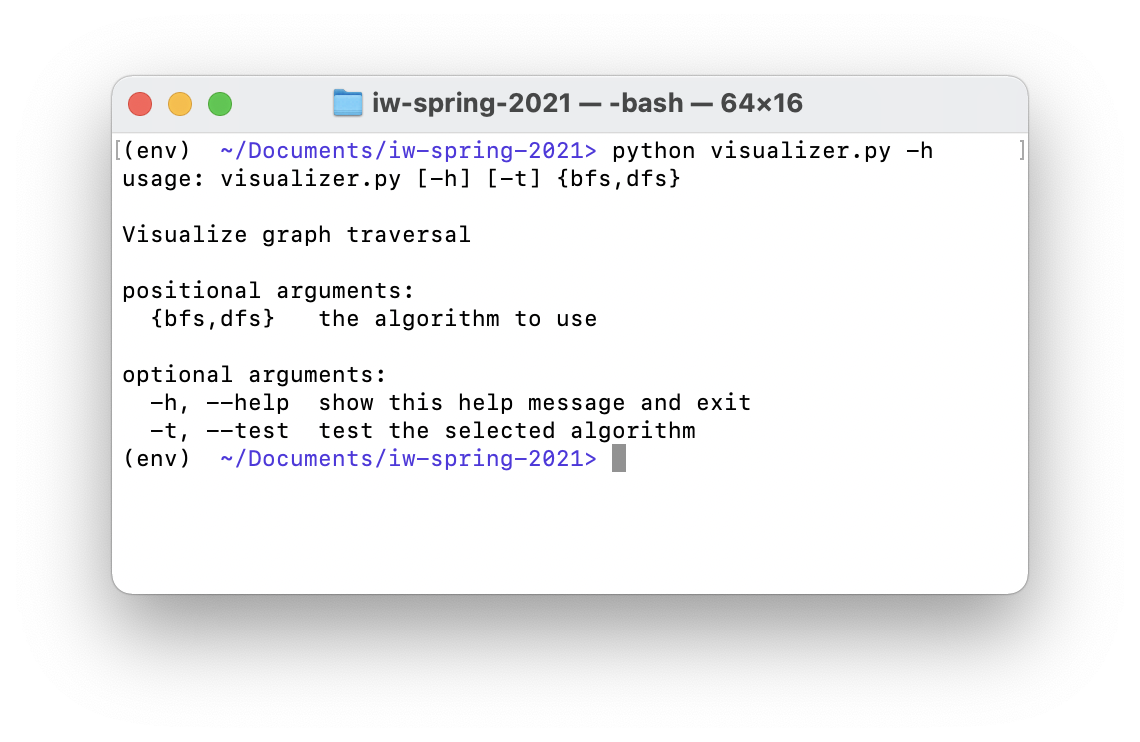
\includegraphics[width=0.75\linewidth]{argparse.png}
\caption{Interacting with the visualizer through the terminal}
\label{fig:argparse}
\end{figure}

Once a valid command is given to the visualizer, a new window will appear on the screen. The graph is drawn and updated using the helper functions provided by the \texttt{Node} class. Once the visualizer has launched, this screen remains the main point of interaction for the student until the visualization finishes. During program execution, all user input is handled through Pygame. The visualizer additionally uses a state machine to manage the current game state. Each possible state is described by a \texttt{GameState} class, which as Listing~\ref{lst:states} illustrates also uses enumeration.

\begin{listing}[hbt]
\centering
\begin{minipage}{0.8\textwidth}%
\linespread{1.0}
\caption{The \texttt{draw()} function}
\begin{minted}[linenos,frame=lines,escapeinside=||]{python}
# All possible gamestates
class GameState(Enum):
	INPUT = auto()
	DEMO = auto()
	TEST = auto()
	END = auto()
\end{minted}
\label{lst:states}
\end{minipage}
\end{listing}

When \texttt{visualizer.py} is run, the program first parses each argument from the command line. Internally, these parameters are used later on to load the reference solution that is required (and the student solution if requested by the user). After the window and graph are created, the visualizer sets the initial game state to \texttt{INPUT} and enters the main game loop. While in this state, students are able to interact with the visualizer regardless of whether they are testing their own implementation or only demonstrating the reference solution.

Students can block or unblock nodes using the mouse. These two actions are handled by the same function, \texttt{handleMouseClick()}, which takes as arguments the current position of the mouse, the node that was clicked, and a type to set the clicked node to. Accessing the clicked \texttt{Node} is accomplished by using the mouse position as an index into the two-dimensional array that makes up the graph. To create a valid index, this requires using integer division to floor these coordinates to that of the nearest \texttt{Node}. Afterwards, the node type can be updated directly before updating the screen. Listing~\ref{lst:mouse} illustrates this operation.

\begin{listing}[hbt]
\centering
\begin{minipage}{0.8\textwidth}%
\linespread{1.0}
\caption{Finding and manipulating a clicked \texttt{Node}}
\begin{minted}[linenos,frame=lines,escapeinside=||]{python}
# Interact with selected node
def handleMouseClick(x, type, graph, screen):
	t = x[0]
	w = x[1]
	g1 = t // (WIDTH // COLS)
	g2 = w // (HEIGHT // ROWS)
	node = graph[g1][g2]
	if (node.type != Node.NodeType.START 
		and node.type != Node.NodeType.GOAL):
			node.type = type
			node.draw(screen)
\end{minted}
\label{lst:mouse}
\end{minipage}
\end{listing}

As described previously, the size of each \texttt{Node} on the screen is made smaller by the \texttt{BORDER} variable. The code for handling mouse clicks avoids the issue of clicking the white space between individual nodes, because each click is effectively mapped to the actual grid area that each node represents.

The game state can be moved forward by pressing the \keystroke{Space} key (e.g. $\texttt{INPUT} \rightarrow \texttt{DEMO}$). The \texttt{TEST} state is skipped if the visualizer is run with only the desired algorithm as an argument. After the \texttt{END} state is reached, the visualizer will remain idle until it is exited by either pressing the \keystroke{Space} key again or by manually closing the game window. Figure~\ref{fig:side-a} illustrates the \texttt{INPUT} state when the visualizer is first opened, and Figure~\ref{fig:side-b} shows the \texttt{DEMO} state after the graph has been changed by the user.

\begin{figure}[hbt]
\begin{minipage}[b]{0.5\linewidth}
\centering
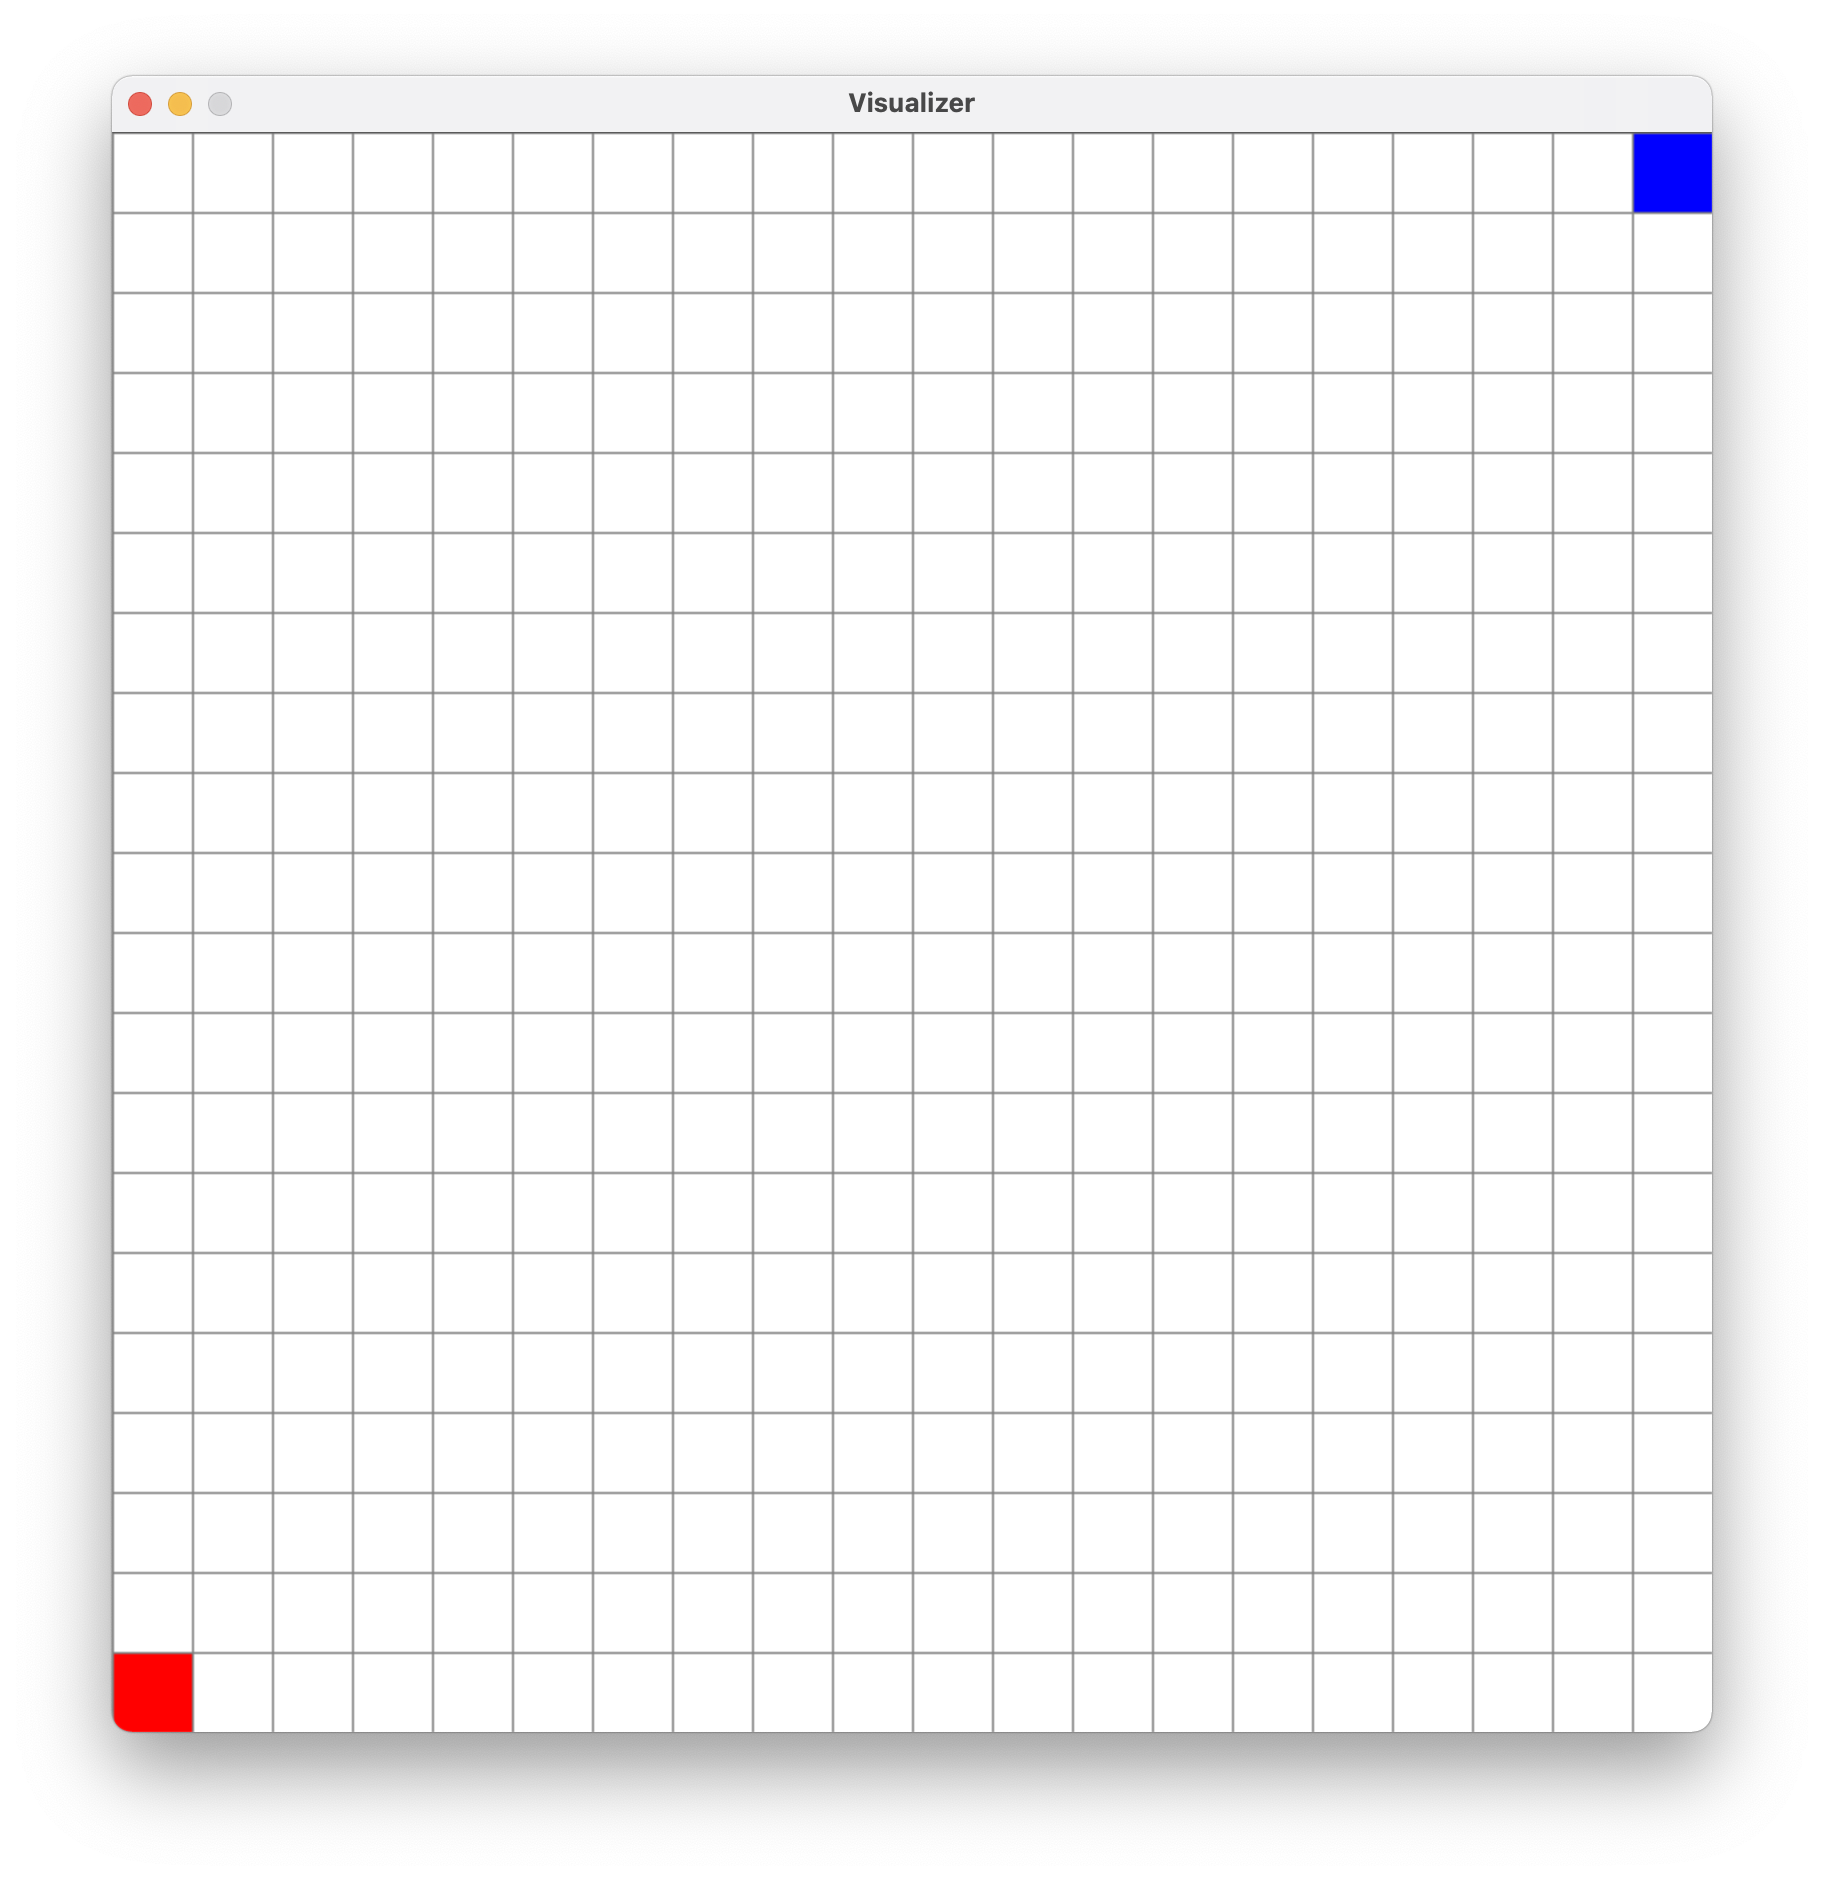
\includegraphics[width=.75\linewidth]{input_state.png}
\caption{The \texttt{INPUT} state}
\label{fig:side-a}
\end{minipage}
\hspace{0.5cm}
\begin{minipage}[b]{0.5\linewidth}
\centering
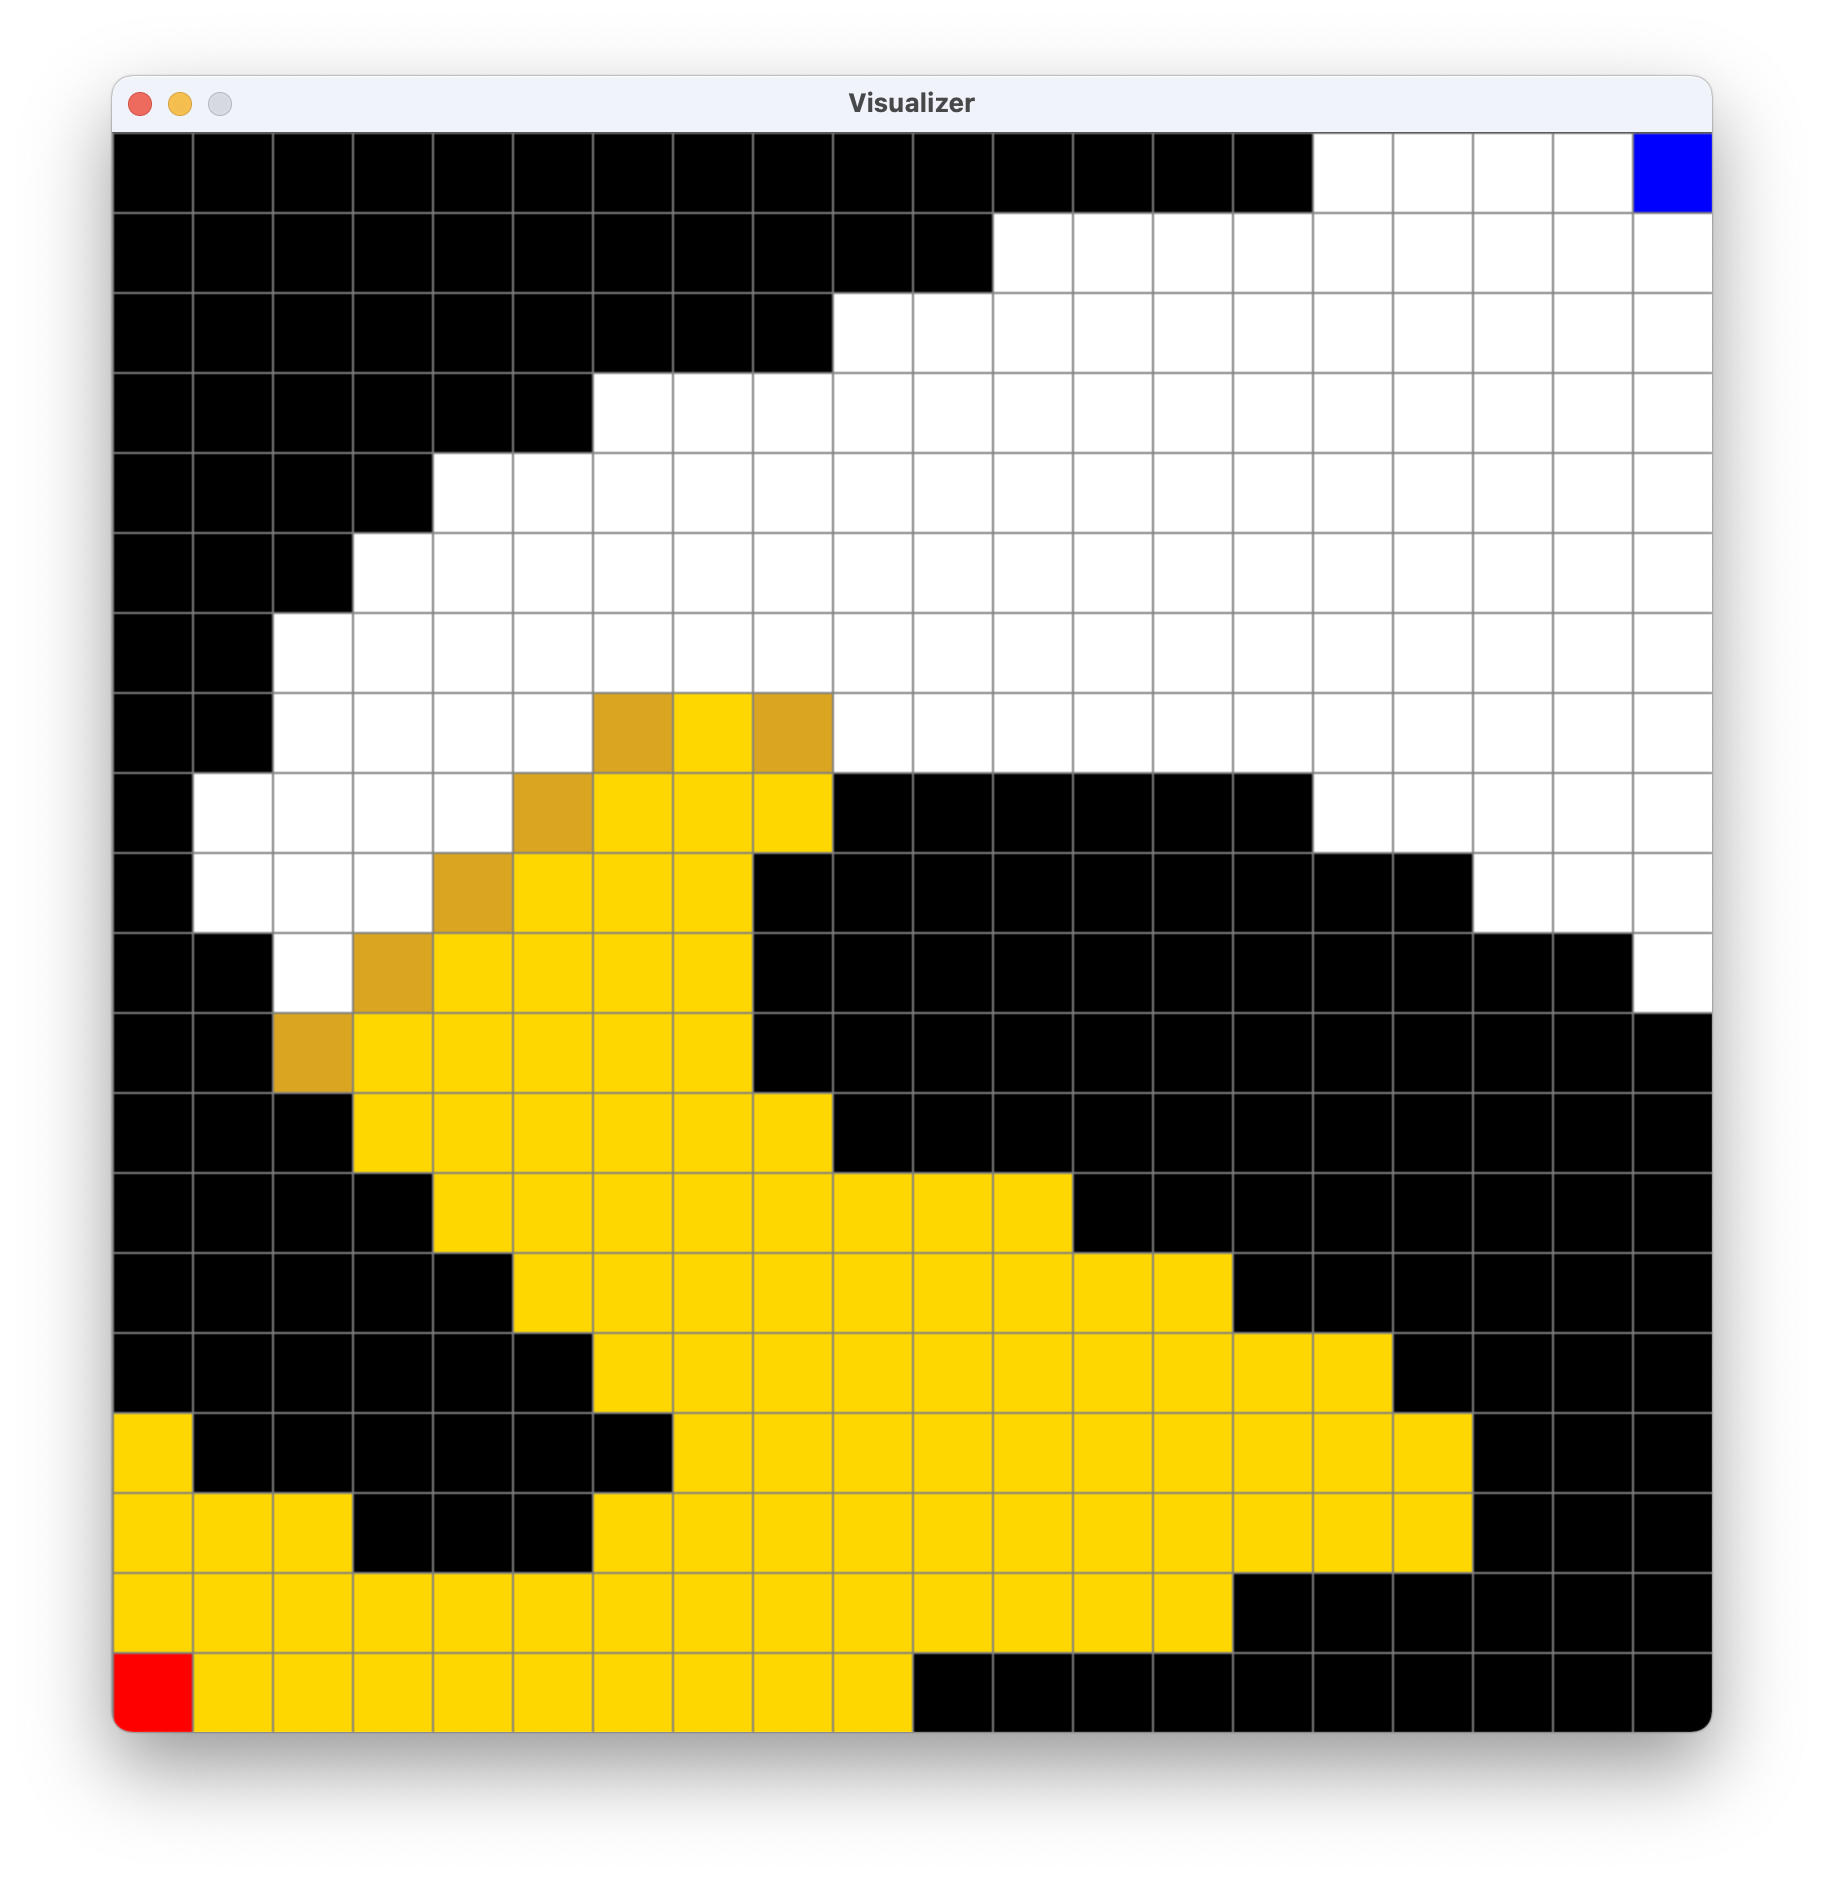
\includegraphics[width=.75\linewidth]{demo_state.png}
\caption{The \texttt{DEMO} state}
\label{fig:side-b}
\end{minipage}
\end{figure}

Students write their implementation of each strategy in a separate file called \texttt{solutions.py}. This Python script declares the function signature of each traversal algorithm, but leaves the implementation details for the assignment to explain. After a student has written a solution for a particular algorithm, they can run the visualizer with the appropriate argument and the \texttt{-t} or \texttt{-{}-test} flag. This triggers the visualizer to demonstrate the chosen algorithm as normal, before loading the student implementation from \texttt{solutions.py} and then comparing the output. Listing~\ref{lst:solutions} shows the solutions file as it is first seen by students.

\begin{listing}[hbt]
\centering
\begin{minipage}{0.8\textwidth}%
\linespread{1.0}
\caption{The initial contents of \texttt{solutions.py}}
\begin{minted}[linenos,frame=lines,escapeinside=||]{python}
# Depth-first search
def dfs(node, explored):
	pass

# Breadth-first search
def bfs(start, goal):
	pass
\end{minted}
\label{lst:solutions}
\end{minipage}
\end{listing}

During development, I decided to leave out any comments explaining the purpose, arguments, and return type of each function. While I initially wanted to include this information, there were a few constraints that made this overly difficult. Unlike C or Java, Python is duck typed. The language allows for objects to be typed, but the same is not true for variables. At the same time, the options for documenting code within a source file are limited. Java, for example, supports \emph{doc comments} which can identify arguments with \texttt{@param} and the return value with \texttt{@return}. This information, along with a description of a function, supports conversion into a fully-documented API that can be hosted online. In contrast, Python's \emph{docstrings} have no special markup and are limited in usefulness by the language's type system. As a result, I chose to move all explanation of the code into the assignment specification with the intention of providing more clarity to students.

\subsection{Assignment Creation}

Although visualization was a critical part of my work, an equally important consideration was the teaching aspect of the project. While it was clear that a formal assignment would be able to carry out this task, it was still necessary to decide what was important to teach and how that content would be taught.

When writing the assignment specification, I took care to structure it in a thoughtful way. Because I intended the assignment to be accessible to a wide audience, the difficulty needed to remain manageable throughout. As a result, I chose to break the assignment into sections that flowed into one another. Upon completion of the installation process for their specific operating system, students are given a brief overview of graph theory and its role in the assignment. Ultimately, students are guided towards implementing their own versions of each traversal algorithm.

The assessment portion is divided between the two algorithms. For both depth-first search and breadth-first search, students are first tasked with exploring the algorithm using the visualizer. This allows a student to familiarize themselves with how the algorithm behaves and reacts to user input before even writing any code. The next task is to actually implement the algorithm in question, given pseudocode that abstractly describes its logic. When necessary, the specification gives additional hints that clarify the requirements of the assignment or emphasize Python fundamentals that might be useful. Finally, students are asked to take their solutions and test them using the visualizer.

The assignment teaches depth-first search before breadth-first search. This placement came after examining each algorithm from a student's perspective. By starting with depth-first search, the intention was to start with a simpler task first before moving onwards to breadth-first search. Using a recursive approach, depth-first search only requires five lines of code (from the reference solution) to return all reachable nodes from a starting point. While recursion is worthy of study on its own, the pseudocode given to the student and the simplicity of just traversing the graph makes the task relatively straightforward. Implementing breadth-first search, on the other hand, requires more complicated logic and a good understanding of Python list methods. Teaching breadth-first search last also establishes how graph traversal algorithms might be used to solve real problems. Students quickly see how breadth-first search is able to return the shortest path between two points.

\subsection{Student Assessment}

In order to assess student understanding, the assignment employs both qualitative and quantitative metrics. In the vein of many current computer science classes at Princeton University, students are asked to fill out a submission file during the assignment. This file, \texttt{submission.md}, is a Markdown document containing a personal questionnaire, written response questions, and a feedback section. While the questionnaire and feedback portions serve to help evaluate the assignment, the written response questions exist specifically to assess students. After a student has explored an algorithm, the corresponding question\footnote{There is actually a third written response question in the final version of \texttt{submission.md}. This question acts as a bonus for students who feel especially comfortable with the material, and asks what change would be needed to implement depth-first search using an iterative approach.} gives them an opportunity to reflect critically and explain its behavior in their own words.

While the written response section enables qualitative assessment of students, it is supplemented by an equally important quantitative assessment of each student's code. As previously described, students are able to test their own implementations of each algorithm by running the visualizer with the \texttt{-t} or \texttt{-{}-test} flag. The visualizer implements a basic autograder that will check for the following conditions:

\begin{itemize}[leftmargin=3cm,font=\textnormal]
\item \emph{The student's solution exists for the given algorithm}
\item \emph{The returned value is of the correct type (a list of nodes)}
\item \emph{The length of the returned list is correct}
\item \emph{Each returned \texttt{Node} is unique}
\item \emph{All reachable nodes were found (depth-first search)}
\item \emph{The shortest path to the goal was found (breadth-first search)}
\end{itemize}

If one of these conditions is violated, the visualizer will show a descriptive error message on the screen and close the game window the next time the \keystroke{Space} key is pressed. Likewise, if the student's implementation passes all tests a message will show to indicate success. Messages are also used to indicate if no path exists to the goal node (such as when the user has blocked all potential paths). Figure~\ref{fig:success} illustrates the success message shown after testing breadth-first search, and Figure~\ref{fig:failure} shows the error message produced from no path existing between the start and goal nodes. By keeping all error messages to the game window, my intention was to prevent students from having to split their attention between the terminal and the visualizer. Additionally, I hoped to provide better error messages than a normal stack trace might offer.

\begin{figure}[hbt]
\begin{minipage}[b]{0.5\linewidth}
\centering
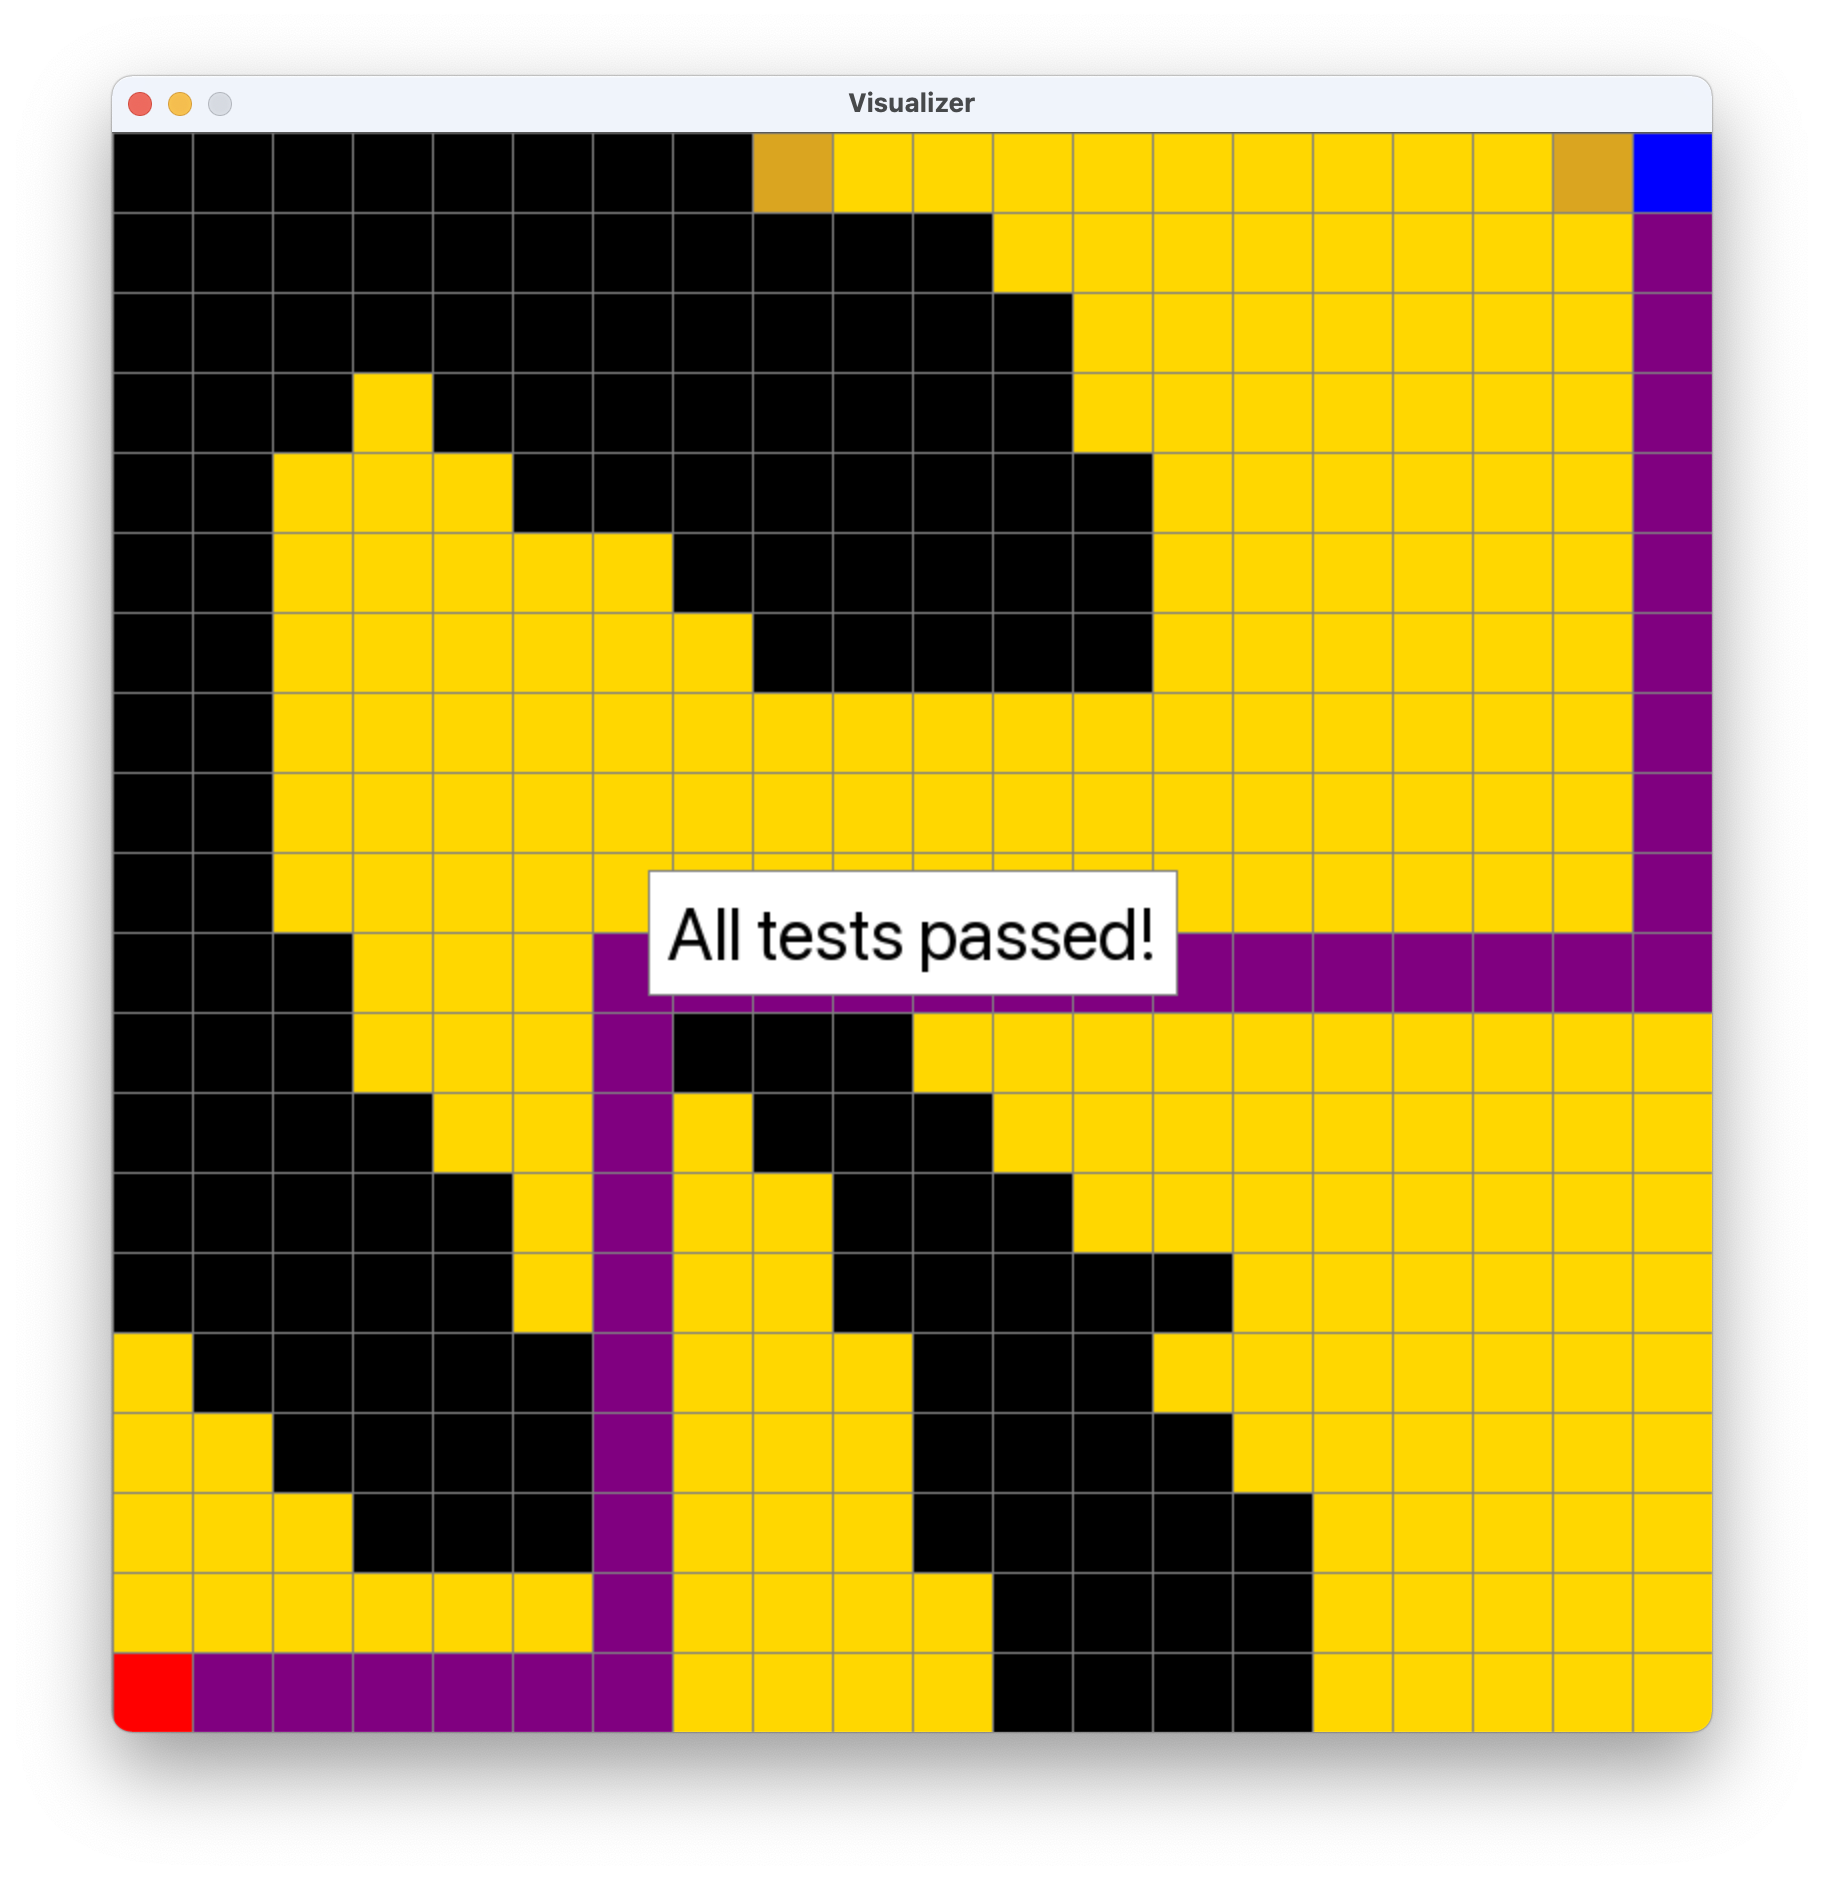
\includegraphics[width=.75\linewidth]{success.png}
\caption{A success message}
\label{fig:success}
\end{minipage}
\hspace{0.5cm}
\begin{minipage}[b]{0.5\linewidth}
\centering
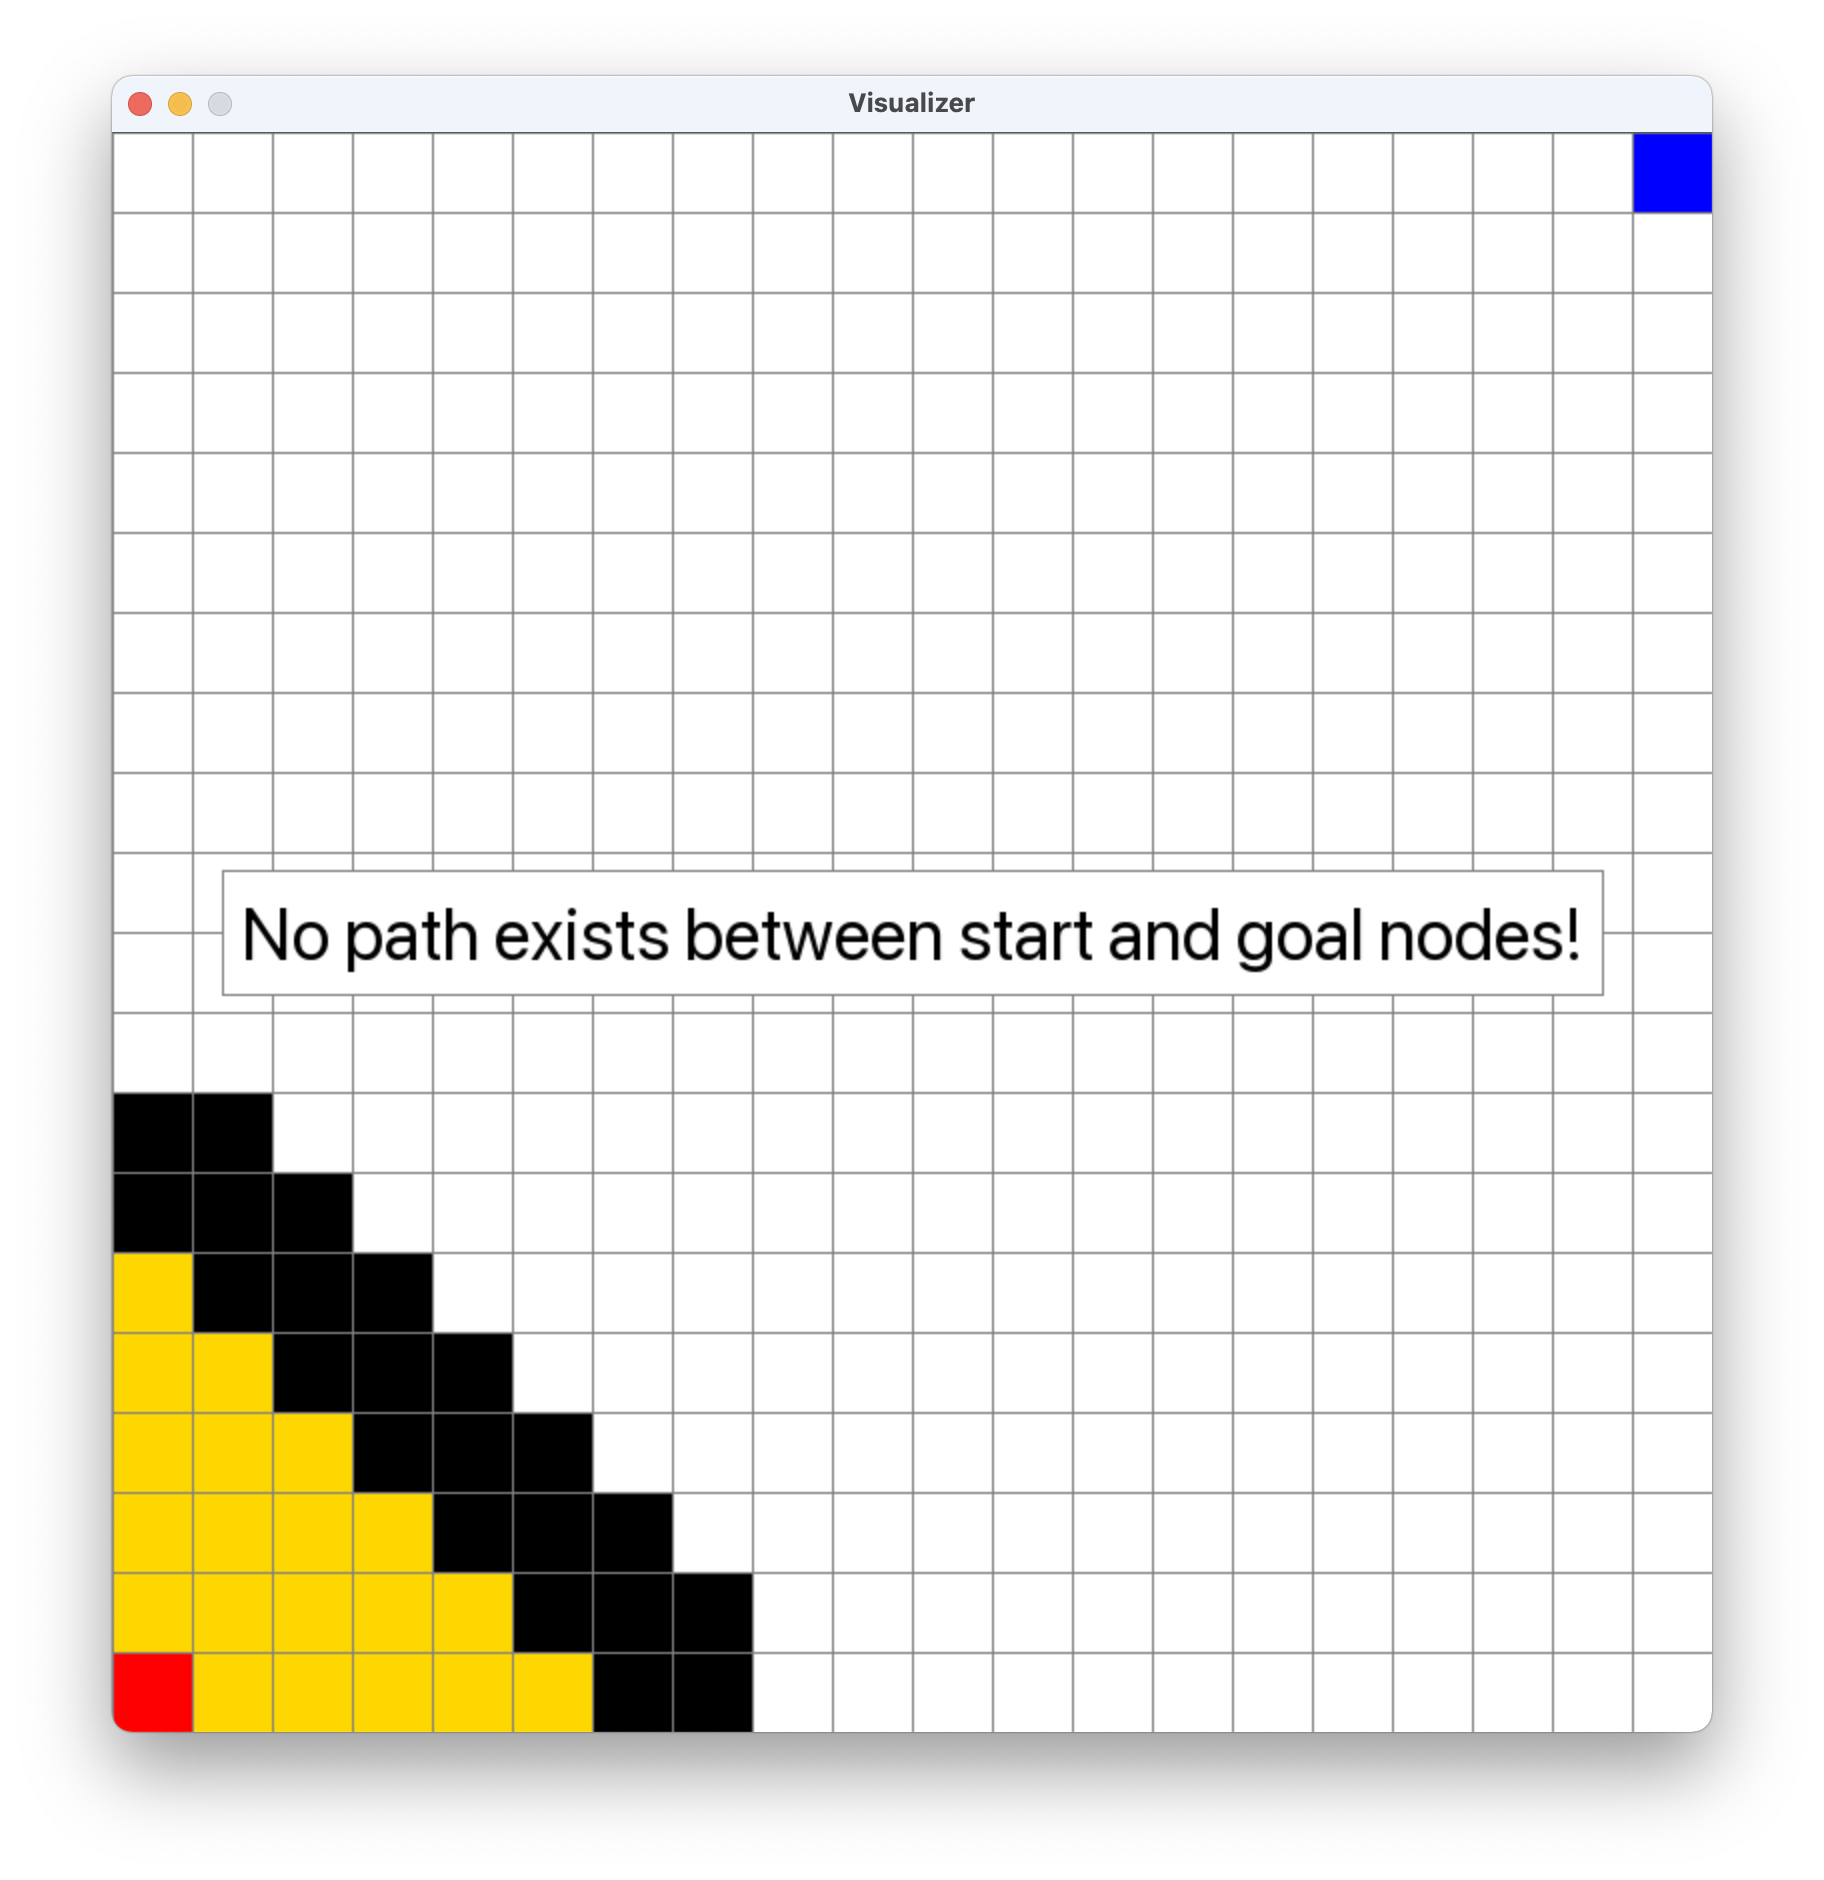
\includegraphics[width=.75\linewidth]{failure.png}
\caption{An error message}
\label{fig:failure}
\end{minipage}
\end{figure}

As an additional measure to validate completion of the assignment, students are asked to upload screenshots that show each of their solutions passing all tests. This is intended to assist a hypothetical professor or TA who might want to quickly check assignment completion. Of course, confirming that a student's solutions are correct is as simple as cloning their repository and running the visualizer.

\section{Evaluation}

\subsection{Evaluation Logistics}

Because the goal of my project was to teach graph traversal algorithms, it was important to actually evaluate it with real students. By advertising the project on various Princeton mailing lists, I sought to cast a wide net and solicit a diverse group of participants to test the assignment. Once the final specification was written, an advertisement was circulated on the \emph{FIRSTCOMEFIRSTSERV}, \emph{butlerbuzz}, and \emph{csugrad} listservs during the week of April 19th, 2021. The first two mailing lists correspond to First College and Butler College respectively, and were included to target a broader audience of Princeton undergraduates. The third list, \emph{csugrad}, is specific to computer science majors at Princeton.

To further incentivize students, each selected participant was compensated with \$50. This sum would be sent through Venmo, a mobile payment service, upon completion of the assignment. While the initial email received over fifty replies, only ten students were invited to participate given my own financial restrictions. Each participant was given a full week to complete the assignment (until Wednesday, April 28th) with nine students ultimately succeeding in this task. In sum, a total of \$450 was spent during the evaluation period.

\subsection{Quantitative Evaluation}

Figure~\ref{fig:breakdown} gives an overview of the final participant cohort (that is to say all students who finished the assignment). The overwhelming majority were computer science majors, and all participants were in a STEM field. While I intended to have more participants from other concentrations, the breakdown of participants by class year does offer a more optimistic picture. The second chart shows that participants were spread fairly evenly between the classes of 2023, 2022, and 2021. Students came in with a range of experience levels and comfort with algorithms, meaning  their feedback would ultimately reflect a wider range of perspectives.

\begin{figure}[hbt]
\centering
\usetikzlibrary {shadows}
\begin{tikzpicture}
\pie[text = inside,color={green!70!black,orange!70,red!70},style=drop shadow]{
77.78/COS,
11.11/ECE,
11.11/PHY
}
\pie[text = inside,pos = {7.5,0},style=drop shadow]{
44.44/2023,
22.22/2022,
33.33/2021
}
\end{tikzpicture}
\caption{Percentage of participants by major and class year}
\label{fig:breakdown}
\end{figure}

Overall response to the assignment was extremely positive. Among all participants, the average rating of the assignment was an 8 out of 10. Crucially, students also rated the specification and the visualizer highly. While I initially worried that the assignment would be too lengthy, especially given that it was released at the end of the semester, the average participant required only around an hour to complete it. Again, this can be partly attributed to students having prior knowledge of computing fundamentals. The average participant, for example, rated both their experience with Python and their experience with algorithms as greater than 6 out of 10. In total, students were asked to give a numeric response to six feedback categories, as illustrated by Table~\ref{table:averages}.

\begin{table}[hbt]
\centering
\begin{tabular}{|l|l|}
\hline
Feedback Category & Average (thousandths) \\
\hline
\hline
Python Experience (1-10) & 6.667 \\
 \hline
Algorithms Experience (1-10) & 6.778 \\
\hline
Assignment Length (hours) & 1.130 \\
\hline
Instructions Quality (1-10) & 7.889 \\
\hline
Visualizer Quality (1-10) & 7.778 \\
\hline
Overall Rating (1-10) & 8 \\
\hline
\end{tabular}
\caption{Average values of feedback categories}
\label{table:averages}
\end{table}

\subsection{Qualitative Evaluation}

While numeric values might give immediate feedback on assignment quality, participants also took advantage of the written response section. It was here that I observed a deeper—and ultimately positive—discussion of the assignment. As a whole, participants stated that they enjoyed the assignment. For some participants, it was refreshing just to use Python in lieu of the Java programming used in introductory Princeton computer science. Other participants appreciated the chance to implement depth-first search and breadth-first search during an assignment. 

Interestingly, multiple students reported that while these algorithms are taught in COS 226, Princeton's algorithms and data structures class, neither is actually implemented by students during the course. This aligns with another repeated observation, namely that COS 226 often describes a particular algorithm without ever showing it in action. Overall, the vast majority of participants reacted positively to the visualization aspect of the assignment. Many felt that the ability to change the graph by blocking or unblocking nodes improved the self-learning experience in a way that a slide deck could not.

However, participants also gave valuable critique on aspects that they felt needed improvement. In particular, the performance of the visualizer was not consistent across different computers. Some users reported that the visualizer ran so quickly that it was impossible to trace what was actually happening. Unfortunately, my decision to use Pygame is partly to blame for this. Pygame is so low-level that it is up to the programmer to implement key timing controls. The recursive nature of depth-first search also made it difficult to use delays as a means of control to the point that these delays were removed in the final code.

In terms of the assignment specification, at least three participants found parts of the instructions confusing. When first released, the assignment did not specify the return type of the functions in \texttt{solutions.py}. Additionally, the pseudocode for each algorithm was made somewhat confusing by the ordering of steps used. This was a limitation of Markdown, because the format only supports nesting lists to the second level. It would have been preferable to write these sections in pure HTML, in order to maintain tighter control over the final markup.

Finally, two participants stated that their previous knowledge of graph theory actually made the visualizer less intuitive for them. While they each said that the visualizer might make a good introduction, the use of a grid with implied edges was less understandable to more experienced programmers. This raises an interesting question, because there is no best way to balance accessibility and adherence to formal theory.

\section{Conclusions and Future Work}

Making a good assignment is difficult. The challenge is the need to not only evaluate the student but the assignment as well. I started this independent work without knowing what exactly to expect. With the evaluation period complete, however, I am satisfied in what I was able to achieve. My project was successful in developing an application and an assignment that worked better together. Real Princeton students used my project to learn something, and I myself learned how to teach them. Not only do I feel more confident in my mastery of these algorithms, but I also feel empowered to share this knowledge with others.

In spite of this reflection, there is still much that can be done. The current codebase, for example, could be altered to improve the stability and performance of the visualizer. Perhaps students might benefit from a browser-based solution, where code could be written in a web app instead of having to install a local version. Another route might lay in adapting the project to other topics. While graph traversal benefits greatly from visualization, it is far from the only candidate for this teaching method.

\section*{Acknowledgements}

This report marks the end of my independent work this semester and the end of my third year at Princeton. Looking back, I am amazed at how far I have come and I owe this progress to everyone who has supported me these past few months. I graciously thank my adviser, Professor David Walker, for enabling me to undertake this project. I also thank my friend, Epi Torres-Smith '22, for testing the assignment specification and giving invaluable feedback throughout the semester. Finally, I thank my family. Their tireless support keeps me moving forward at a time when the rest of the world seems to stand still.

\section*{Honor Code}

I pledge my honor that this paper represents my own work in accordance with University regulations \\/s/ William Svoboda

\pagebreak

\bstctlcite{bstctl:etal, bstctl:nodash, bstctl:simpurl}
\bibliographystyle{IEEEtranS}
\bibliography{references}

\appendix

\section{Appendix}

All project code is hosted on GitHub at \url{https://github.com/disstillwill/IW-Spring-2021} along with the assignment specification. The assignment website can be accessed directly at \url{https://disstillwill.github.io/IW-Spring-2021/} or from the project repository.

\end{document}

